\chapter[Foes'-fear]{
    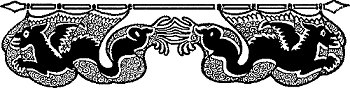
\includegraphics[width=9.3cm]{viking-tales/020}\\
    Foes'-fear}

\lettrine{E}{very} day the boy Harald heard some such story of war or of
the gods, until he could see Thor riding among the storm-clouds and
throwing his hammer, until he knew that a brave man has many wounds, but
never a one on his back. Many nights he dreamed that he himself walked
into Valhalla, and that all the heroes stood up and shouted:

``Welcome! Harald Halfdanson!''

``Ah! the bite of the sword is sweeter than the kiss of your mother,''
he said to Olaf one day. ``When shall I stand in the prow of a dragon
and feast on the fight? I am hungry to see the world. Ivar the Far-goer
tells me of the strange countries he has seen. Ah! we vikings are great
folk. There is no water that has not licked our boats' sides. This cape
of mine came in a viking boat from France. These cloak-pins came from a
far country called Greece. In my father's house are golden cups from
Rome, away on the southern sea. Every land pours rich things into our
treasure-chest. Ivar has been to a strange country where it is all sand
and is very hot. The people call their country Arabia. They have never
heard of Thor or Odin. Ivar brought beautiful striped cloth from there,
and wonderful, sweet-smelling waters. Oh! when shall the white horses of
the sea lead me out to strange lands and glorious battles?''

But Harald did something besides listen to stories. Every morning he was
up at sunrise and went with a thrall to feed the hunting dogs. Thorstein
taught him to swim in the rough waters of the fiord. Often he went with
the men a-hunting in the woods and learned to ride a horse and pull a
bow and throw a lance. Ivar taught him to play the harp and to make up
songs. He went much to the smithy, where the warriors mended their
helmets and made their spears and swords of iron and bronze. At first he
only watched the men or worked the bellows, but soon he could handle the
tongs and hold the red-hot iron, and after a long time he learned to use
the hammer and to shape metal. One day he made himself a spear-head. It
was two feet long and sharp on both edges. While the iron was hot he
beat into it some runes. When the men in the smithy saw the runes they
opened their eyes wide and looked at the boy, for few Norsemen could
read.

``What does it say?'' they asked.

``It is the name of my spear-point, and it says, `Foes'-fear,''' Harald
said. ``But now for a handle.''

It was winter and the snow was very deep. So Harald put on his skees and
started for a wood that was back from shore. Down the mountains he went,
twenty, thirty feet at a slide, leaping over chasms a hundred feet
across. In his scarlet cloak he looked like a flash of fire. The wind
shot past him howling. His eyes danced at the fun.

``It is like flying,'' he thought and laughed. ``I am an eagle. Now I
soar,'' as he leaped over a frozen river.

He saw a slender ash growing on top of a high rock.

``That is the handle for `Foes'-fear,''' he said.

The rock stood up like a ragged tower, but he did not stop because of
the steep climb. He threw off his skees and thrust his hands and feet
into holes of the rock and drew himself up. He tore his jacket and cut
his leather leggings and scratched his face and bruised his hands, but
at last he was on the top. Soon he had chopped down the tree and had cut
a straight pole ten feet long and as big around as his arm. He went
down, sliding and jumping and tearing himself on the sharp stones. With
a last leap he landed near his skees. As he did so a lean wolf jumped
and snapped at him, snarling. Harald shouted and swung his pole. The
wolf dodged, but quickly jumped again and caught the boy's arm between
his sharp teeth. Harald thought of the spear-point in his belt. In a
wink he had it out and was striking with it. He drove it into the wolf's
neck and threw him back on the snow, dead.

``You are the first to feel the tooth of `Foes'-fear,''' he said, ``but
I think you will not be the last.''

\begin{figure}
    \centering
    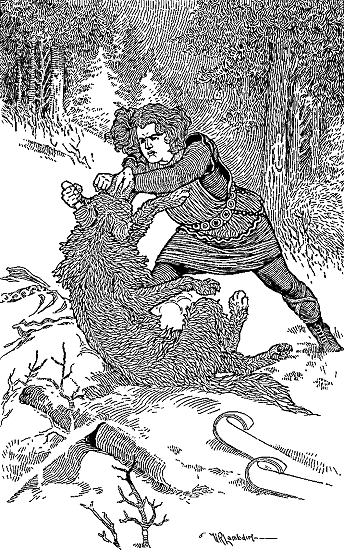
\includegraphics[width=9.1cm]{viking-tales/021}
    \caption{``He drove it into the wolf's neck''}
\end{figure}

Then without thinking of his torn arm he put on his skees and went
leaping home. He went straight to the smithy and smoothed his pole and
drove it into the haft of the spear-point. He hammered out a gold band
and put it around the joining place. He made nails with beautiful heads
and drove them into the pole in different places.

``If it is heavy it will strike hard,'' he said.

Then he weighed the spear in his hand and found the balancing point and
put another gold band there to mark it.

Thorstein came in while he was working.

``A good spear,'' he said.

Then he saw the torn sleeve and the red wound beneath.

``Hello!'' he cried. ``Your first wound?''

``Oh, it is only a wolf-scratch,'' Harald answered.

``By Thor!'' cried Thorstein, ``I see that you are ready for better
wounds. You bear this like a warrior.''

``I think it will not be my last,'' Harald said.
